\documentclass[10pt,conference]{IEEEtran}\usepackage[]{graphicx}\usepackage[table,xcdraw]{xcolor}
% maxwidth is the original width if it is less than linewidth
% otherwise use linewidth (to make sure the graphics do not exceed the margin)
\makeatletter
\def\maxwidth{ %
  \ifdim\Gin@nat@width>\linewidth
    \linewidth
  \else
    \Gin@nat@width
  \fi
}
\makeatother

\definecolor{fgcolor}{rgb}{0.345, 0.345, 0.345}
\newcommand{\hlnum}[1]{\textcolor[rgb]{0.686,0.059,0.569}{#1}}%
\newcommand{\hlstr}[1]{\textcolor[rgb]{0.192,0.494,0.8}{#1}}%
\newcommand{\hlcom}[1]{\textcolor[rgb]{0.678,0.584,0.686}{\textit{#1}}}%
\newcommand{\hlopt}[1]{\textcolor[rgb]{0,0,0}{#1}}%
\newcommand{\hlstd}[1]{\textcolor[rgb]{0.345,0.345,0.345}{#1}}%
\newcommand{\hlkwa}[1]{\textcolor[rgb]{0.161,0.373,0.58}{\textbf{#1}}}%
\newcommand{\hlkwb}[1]{\textcolor[rgb]{0.69,0.353,0.396}{#1}}%
\newcommand{\hlkwc}[1]{\textcolor[rgb]{0.333,0.667,0.333}{#1}}%
\newcommand{\hlkwd}[1]{\textcolor[rgb]{0.737,0.353,0.396}{\textbf{#1}}}%
\let\hlipl\hlkwb

\usepackage{framed}
\makeatletter
\newenvironment{kframe}{%
 \def\at@end@of@kframe{}%
 \ifinner\ifhmode%
  \def\at@end@of@kframe{\end{minipage}}%
  \begin{minipage}{\columnwidth}%
 \fi\fi%
 \def\FrameCommand##1{\hskip\@totalleftmargin \hskip-\fboxsep
 \colorbox{shadecolor}{##1}\hskip-\fboxsep
     % There is no \\@totalrightmargin, so:
     \hskip-\linewidth \hskip-\@totalleftmargin \hskip\columnwidth}%
 \MakeFramed {\advance\hsize-\width
   \@totalleftmargin\z@ \linewidth\hsize
   \@setminipage}}%
 {\par\unskip\endMakeFramed%
 \at@end@of@kframe}
\makeatother

\definecolor{shadecolor}{rgb}{.97, .97, .97}
\definecolor{messagecolor}{rgb}{0, 0, 0}
\definecolor{warningcolor}{rgb}{1, 0, 1}
\definecolor{errorcolor}{rgb}{1, 0, 0}
\newenvironment{knitrout}{}{} % an empty environment to be redefined in TeX

\usepackage{alltt}
%\IEEEoverridecommandlockouts
% The preceding line is only needed to identify funding in the first footnote. If that is unneeded, please comment it out.
\usepackage{cite}
\usepackage{amsmath,amssymb,amsfonts}
\usepackage{algorithmic}
\usepackage{graphicx}
\usepackage{textcomp}
\usepackage{xcolor}
\usepackage{hyperref}
\usepackage{listings}
\usepackage{enumitem}
\usepackage{placeins}
\usepackage{caption}
\usepackage{subcaption}
\usepackage{multirow}
\usepackage{graphicx}
\usepackage[table,xcdraw]{xcolor}

% Definitions for listings
\definecolor{dkgreen}{rgb}{0,0.6,0}
\definecolor{gray}{rgb}{0.5,0.5,0.5}
\definecolor{mauve}{rgb}{0.58,0,0.82}
\lstset{frame=none, % tblr
  language=R,
  escapeinside={\%*}{*)},          % if you want to add LaTeX within your code
  aboveskip=3mm,
  belowskip=3mm,
  showstringspaces=false,
  columns=flexible,
  basicstyle={\footnotesize\ttfamily},
  numbers=none,
  numberstyle=\tiny\color{gray},
  keywordstyle=\color{blue},
  commentstyle=\color{dkgreen},
  stringstyle=\color{mauve},
  breaklines=true,
  breakatwhitespace=true,
  tabsize=3,
  moredelim=[is][\sout]{¡}{¡},
}

% Commands
\newcommand{\odnote}[1]{[\textcolor{blue}{NOTA OSCAR: #1]~}}
\newcommand{\etal}[0]{~\textit{et al.}}
\newcommand{\here}[0]{\textcolor{purple}{-------------SEGUIR AQUI}}
\IfFileExists{upquote.sty}{\usepackage{upquote}}{}
\begin{document}



\title{Which demographic variables better characterize a population?}

\author{
\IEEEauthorblockN{Oscar Dieste}
\IEEEauthorblockA{\textit{Universidad Polit\'ecnica de Madrid}\\
Madrid, Spain \\
odieste@fi.upm.es}
\and
\IEEEauthorblockN{Silvia T. Acu\~na}
\IEEEauthorblockA{\textit{Universidad Aut\'onoma de Madrid}\\
Madrid, Spain \\
silvia.acunna@uam.es}
\and
\IEEEauthorblockN{Natalia Juristo}
\IEEEauthorblockA{\textit{Universidad Polit\'ecnica de Madrid}\\
Madrid, Spain \\
natalia@fi.upm.es}
}

\maketitle

\begin{abstract}
This document is a model and instructions for \LaTeX.
This and the IEEEtran.cls file define the components of your paper [title, text, heads, etc.]. *CRITICAL: Do Not Use Symbols, Special Characters, Footnotes, 
or Math in Paper Title or Abstract.
\end{abstract}

\begin{IEEEkeywords}
component, formatting, style, styling, insert
\end{IEEEkeywords}

\section{Introduction}

Los factores humanos influyen en el proceso de desarrollo de software. Las comunidades científica y profesional generalmente asumen que factores como la experiencia o el conocimiento tienen efectos positivos sobre la X [REFS], Y [REFS] o Z [REFS].

No obstante, existen resultados negativos. \odnote{Ir al paper y quizás a la tesis de Alejandrina, e indicar casos de resultados negativos}

Nuestro objetivo es identificar qué factores humanos son relevantes.

Poner la sección 3 aquí.


\section{Background}\label{sec:background}

\subsection{Related works}

It is unclear which personal aspects influence TDD programming. The most comprehensive review has been performed by Raura\etal{} \cite{} using both primary and secondary studies on TDD. The authors found that the \textit{overall professional experience}, \textit{TDD experience}, \textit{programming language experience}, and \textit{training} were the personal aspects most frequently examined in the empirical research. Evidence is somewhat conflicting, but these personal aspects seem to influence TDD performance positively. A remarkable exception happens when the experience is dichotomized into the \textit{professional} and \textit{student} categories: Professionals seem less productive than students.

During the FiDiPro ESEIL project \cite{juristo2016experiences}, we conducted multiple TDD experiments in Industry and Academy%
\footnote{The experiments conducted during the ESEIL project are described \odnote{Poner una URL correcta} \href{https://docs.google.com/forms/d/1-UGx8xDZ6EWyvAabIvIRWnx7UDIQj1-Ts5w0wBS3UgA}{here}.\label{foot:eseil}}.
We collected the participants' demographic information using a survey%
\footnote{All surveys are available from the URL specified in footnote \#\ref{foot:eseil}. The raw answers are also available in the same URL.}. The surveys evolved during the project, but they all inquired about the participants' education, training, experience, and knowledge from different perspectives, e.g., testing, methodologies, programming languages, etc. Due to the small sample size at the experiment level, we did not individually analyze the influence of the personal aspects on TDD performance (except for Fucci\etal \cite{fucci2015towards}, whose results were inconclusive). 

At the project's end, Dieste\etal \cite{dieste2018empirical} performed a joint analysis.%
\footnote{Due to the characteristics of the special issue where the paper was published, Dieste\etal \cite{dieste2018empirical} only reports the influence of personal factors on ITL (Iterative Test-Last) programming. We report in this paper the influence of personal factors on TDD (see Appendix~\ref{sec:appendix:missing-analyses}). Readers can perform such analyses using the dataset and the SPSS\textsuperscript{\textcopyright} analysis scripts reported in \cite{dieste2018empirical}.}
As far as we know, this is the most extensive study of the impact of personal aspects on TDD performed to date. The analyses yielded a mixture of intuitive and counter-intuitive results:
\begin{enumerate}
     \item \textbf{Intuitive}: When practicing ITL programming, professionals achieve higher quality and productivity than students. Likewise, participants with a degree in Computing exhibit better quality and productivity%
\footnote{The concepts of quality and productivity are intuitive. For a formal definition, see \cite{dieste2018empirical}.}%
.
     \item \textbf{Counter-intuitive}\label{item:counter:2}: When practicing TDD, professionals achieve lower quality and productivity than students. Likewise, participants with a degree in Computing exhibit worse quality and productivity. These results contradict common sense%
\footnote{Please check the statistical significances in Appendix~\ref{sec:appendix:missing-analyses}. Several variables are non-significant, but the trends are clear.}%
, although, as indicated above, \textit{literature reviews on TDD have reported that professionals seem less productive than students}.
     \item \textbf{Intuitive}: The programming experience acquired by the participants during their formal education improves quality and productivity, regardless the participants are using ITL programming or TDD%
\footnote{Statistical significance was not reached for quality when participants performed TDD; see Appendix~\ref{sec:appendix:missing-analyses}.}%
.
     \item \textbf{Counter-intuitive}\label{item:counter:4}: The programming experience acquired by the participants during their formal education is the only experience that influences ITL programming or TDD. However, according to the literature and common sense, \textit{other experiences} should have an effect too, e.g., programming experience acquired in industry.
\end{enumerate}

\subsection{Possible explanations}

Counter-intuitive results should have an explanation. For the item \#\ref{item:counter:2} above, we believe the results are artifactual. Dieste\etal \cite{dieste2017professionals} reports that age is related to a particular type of drop-off characterized by not finalizing the experimental tasks. Senior participants work in the experimental tasks at a slower pace, causing the impression of diminished performance. Ultimately, it is a motivation issue.

The reason for the item \#\ref{item:counter:4} is less obvious. If the academic programming experience has an effect, the industry programming experience should have a (positive) effect as well. Furthermore, the effect of academic programming experience holds both for ITL and TDD, so it does not look like an artifactual effect, i.e., unrelated to senior participants' motivation. In our opinion, two explanations are possible:
\begin{itemize}
     \item \textbf{Experience only sometimes leads to better performance}: McDaniel\etal \cite{mcdaniel1988job} reported low correlations between experience and performance. Camerer and Johnson \cite{camerer1991process} conclude that subjects with experience make decisions or predictions that are no better (or even worse) than those made by inexperienced subjects. There are studies with similar outcomes in programming \cite{muller2004empirical,sheppard1979modern}, as well as in other areas of SE, e.g., \cite{marakas1998semantic,sonnentag1995excellent}. 
     This apparent contradiction can be explained if a distinction is made between experience and expertise. To achieve expert performance, subjects need to complete a period of intensive practice with the deliberate intention of improving performance (i.e., acquiring expertise). The mere exercise of an activity (i.e., the industry programming experience) may improve performance but not to the point of it being equal to that of people generally recognized as experts in an area \cite{ericsson1994expert}.
     \item \textbf{Measurement problem}: Academic programming experience is relatively well-defined. Students do lots of programming in their degrees. However, industry programming experience could be more challenging to estimate. In a regular workday, practitioners meet, answer emails, write reports, and sometimes code. On top of that, different professionals spend different times on each of these activities, and the times evolve over the practitioners' careers.
\end{itemize}

The first explanation has been explored in Dieste\etal \cite{dieste2018empirical}. The authors could not find evidence against it, i.e., such an explanation is consistent with the empirical data. This paper will explore the second explanation, i.e., whether the lack of relationship and superior performance may be due to measurement problems.

\section{Methodology}

\url{https://stats.stackexchange.com/questions/215404/is-there-factor-analysis-or-pca-for-ordinal-or-binary-data}

\url{https://www.youtube.com/watch?v=crbZa5XRVh4}

\subsection{Dataset(s)}\label{sec:dataset}

We collected information about 178 experimental subjects (84 professionals and 94 students). A curated version of the dataset is available at \url{http://www.grise.upm.es/sites/extras/11/}.

\subsection{Measurement problems}

\color{red}

In some cases, e.g., the different types of experience, we requested the same information using different scales (\textit{Likert} and \textit{number of years}) to avoid the risk of bias in the responses \cite{aranda2014evidence}.

\color{black}

\subsection{Research questions}

More concretely, this paper aims to answer the following research questions:

\begin{enumerate}[label=\textbf{RQ\arabic*.~}, align=left]
    \item Is it possible to summarize the data, e.g., pooling together different types of experience so that a ''more solid definition'' of experience shows up? In other words, if we apply a dimension-reduction procedure to the demographic data, does such a procedure yield interpretable results?

    \item Does the dimension-reduced demographic data predict the code quality and programmers' productivity more accurately than the original, non-reduced demographic data?
\end{enumerate}

\subsection{Analysis method}

We will use the Exploratory Factor Analysis (EFA) for dimensionality reduction. The reason is twofold: 1) EFA has been often used in software engineering \cite{siegmund2014measuring,barcomb2019episodic}, and 2) EFA's output can be interpreted as non-observable \textit{constructs} that underlie the experimental data \cite[Chapter 1]{watkins2020step}. The analyses have been conducted with \textit{R}~\cite{R}.

In the realm of Psychology, a construct is \textit{a label for a cluster or domain of covarying behaviours}~\cite{britannicaConstructPsychology}. For instance, intelligent people are expected to perform well on math or language tests. Math and language test scores are ''covarying behaviours'' because they tend to increase/decrease together depending on whether the people are more/less intelligent. Intelligence plays, in this case, the role of construct. 

Outside Psychology, the concept of construct receives other names, such as \textit{latent variable} in Structural Equation Modelling \cite{kline2015principles}. We will use the term ''construct'' because Bacharach's theory components \cite{bacharach1989organizational} are frequently used and well-known in software engineering, e.g., \cite{juristo2013basics,wohlin2012experimentation}.

EFA is frequently used in social sciences to explore the psychometric properties of a survey \cite{costello2005best}. Surveys contain several related questions because it is challenging for a single question to provide the sought information accurately. The EFA helps to identify which queries are associated with the same construct. This is precisely the starting point for this research.

\subsection{Reproducibility}

The demographic data is available online (see Section~\ref{sec:dataset}). The paper in \lstinline{.Rtex} mode (including embedded R code) is be available at \url{ADD GITHUB}.

\section{Results}

We will follow Watkins' guidance \cite[pp. 33]{watkins2020step} to conduct the analysis. It is the best book, in our humble opinion, about EFA. 

The variables in our dataset are binary and ordinal; we will apply polychoric correlations instead of Pearson correlations accordingly.

\subsection{Participants and variables}

The demographic variables are listed in Appendix~\ref{sec:appendix:demographic-variables}.

\subsection{Factorability considerations}

\begin{figure*}[ht]
\centering
\begin{subfigure}{.8\textwidth}
  \centering
\begin{knitrout}
\definecolor{shadecolor}{rgb}{0.969, 0.969, 0.969}\color{fgcolor}
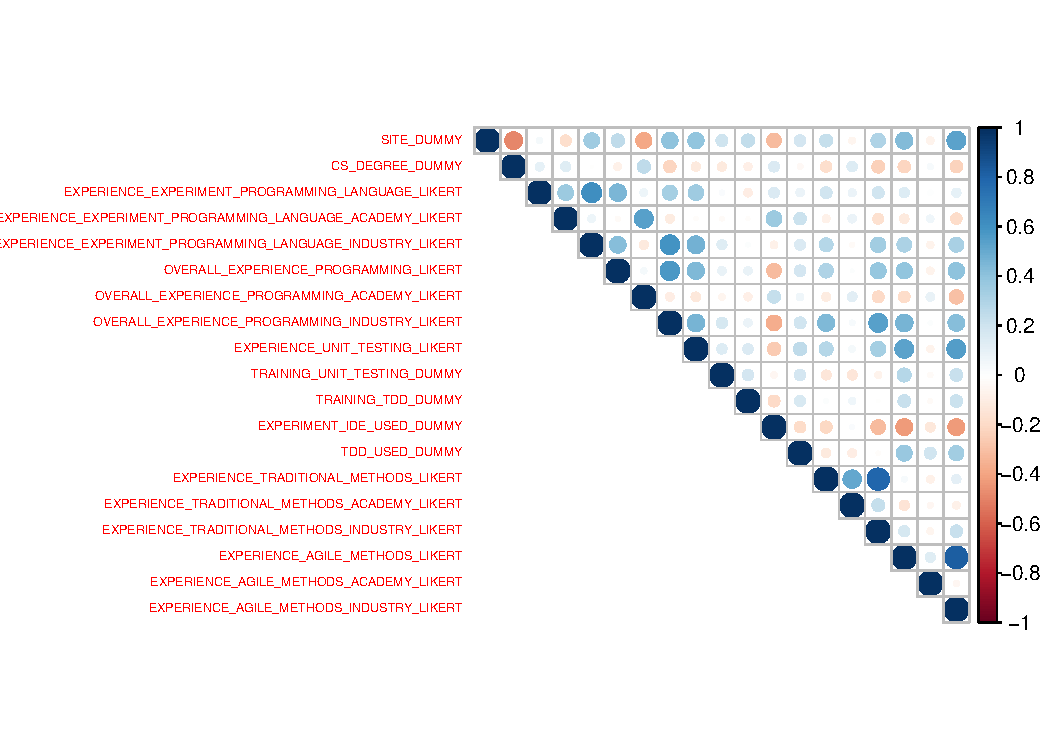
\includegraphics[width=\maxwidth]{figure/correlations_likert-1} 
\end{knitrout}
  \caption{Measured using Likert scales}
  \label{fig:correlations_likert}
\end{subfigure}%
\\
\begin{subfigure}{.8\textwidth}
  \centering
\begin{knitrout}
\definecolor{shadecolor}{rgb}{0.969, 0.969, 0.969}\color{fgcolor}
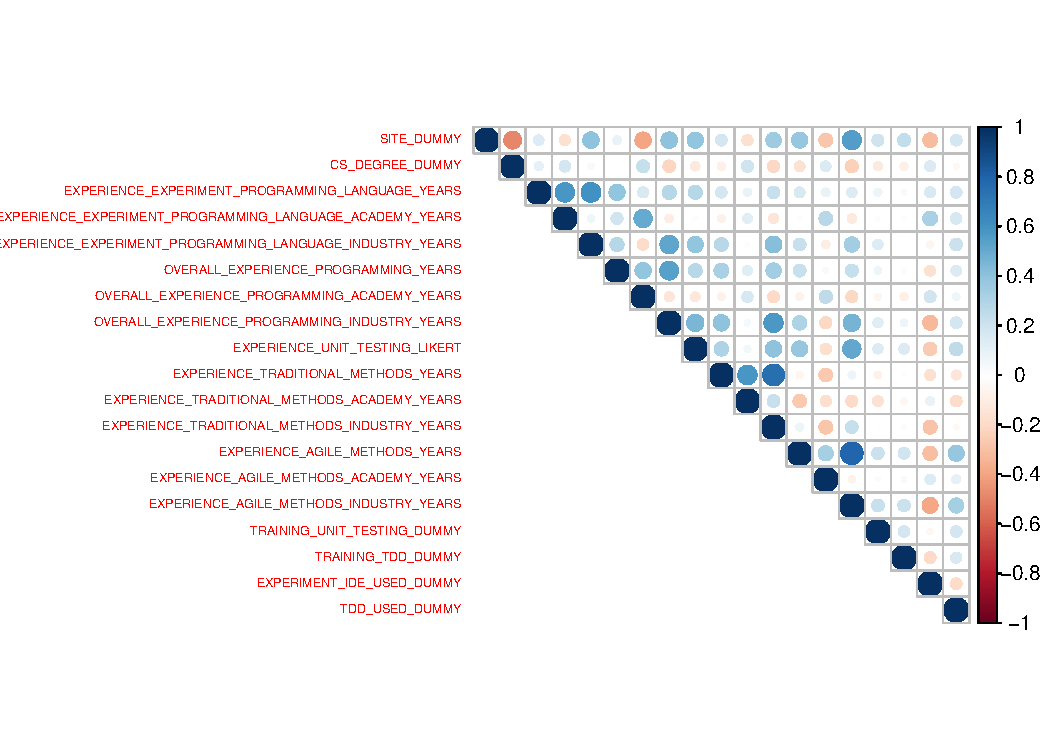
\includegraphics[width=\maxwidth]{figure/correlations_years-1} 
\end{knitrout}
    \caption{Measured using years}
    \label{fig:correlations_years}
\end{subfigure}
\caption{Biserial (Kendall) correlations between demographic variables. We are not using Pearson correlations because some variables, e.g., CS\_DEGREE, are dummies or have been measured in a Likert scale, e.g., EXPERIENCE\_UNIT\_TESTING.}
\label{fig:correlations}
\end{figure*}


Figure~\ref{fig:correlations} shows the biseral correlations 

As a side effect, we obtained somewhat redundant information. For instance, question \#4 about \textit{overall programming experience} subsumes, to some extent, question \#3 regarding the programming languages used by the subject. It was not a surprise that the data were highly correlated, as figures~\ref{fig:correlations_likert} and \ref{fig:correlations_years} show. 

The variables measured in Likert and year scales are also correlated. However, these correlations are not interesting to this research (please note that Figure~\ref{fig:correlations_likert} includes variables measured in a Likert scale and Figure~\ref{fig:correlations_years} variables measured in years). We collected both scales because our previous research showed that students' responses are biased when subjective scales, e.g., a five-point Likert scale (1=low and 5=high), are used \cite{aranda2014evidence}. Other researchers have recently come to similar conclusions \cite{daun2021reliability} (but others not, e.g., \cite{siegmund2014measuring}).

\textcolor{red}{contar aqui lo de los niveles detallado y simplificado}

\FloatBarrier

There are several, sometimes conflicting recommendations to assess the factorability of a dataset. Three criteria frequently mentioned in textbooks are:
\begin{itemize}

    \item There are several correlations with values $r > 0.30$. This fact can be easily assessed by looking at Figure~\ref{fig:correlations}. There are more and higher correlations when the demographic variables are measured in years (Figure~\ref{fig:correlations_years}). Intuitively, that dataset is ''better'', and the final results corroborate this impression. 
    
    \item The determinants of the correlation matrices are 0.0002 and 0.0001). A dataset is not affected by multicollinearity when the determinat $> 0.00001$ \cite[Chapter 9]{watkins2020step}.


    \item The variable/sample size ratio exceeds $1:5$, although some authors recommend higer values ($1:10$ or even $1:20$) \cite{watkins2020step}. The four datasets contain 124 cases, yielding 
    $1:11.3$, 
    $1:11.3$, 
    $1:8.3$, and 
    $1:8.3$ ratios, respectively. 

    \item The Kaiser-Meyer-Olkin (KMO) measure of sampling adequacy estimates the proportion of variance that can be assigned to the underlying constructs \cite{watkins2020step}. EFA can be applied to a dataset when $KMO \geq 0.6$ \cite{kaiser1974little}. The KMO values for our datasets are
    0.7,
    0.65,
    0.7, and
    0.7,
    respectively.


    \item The Bartlett's test of sphericity checks whether the variables in the original dataset are redundant. The null hypothesis states that the variables are not redundant. Dimension reduction is thus possible when Bartlett's test achieves statistical significance (typically at the $\alpha = 0.05$ level) \cite{watkins2020step}. In the four datasets, p-value $< 0.001$.
    
\end{itemize}

\subsection{Number of factors}

The visual examination of the scree plot usually defines the number of factors to extract. However, we have used an alternate approach provided by the \lstinline{fa.parallel()} function from the \lstinline{psych} package \cite{psych}. This function uses the ''parallel'' analysis proposed by Horn \cite{horn1965rationale}. The advantage of the parallel approach vs. scree plot examination is objectivity. Nevertheless, other ''objective'' approaches exist (see, e.g., the help page of the \lstinline{fa.parallel()} function or \cite[Chapter 12]{watkins2020step}).



Datasets 1 -- 3 can be summarized using three factors. In the case of the dataset 4, the function \lstinline{fa.parallel()} suggests four factors\footnote{Due to the randomness that underlies \lstinline{fa.parallel()} (the comparison between the observed data and a random data matrix), in some executions, the suggested number of factors is three.}.

\subsection{Factor extraction}

The factors have been extracted using the \lstinline{fa} function \cite{psych}. We have used Ordinary Least Squares as extraction method because it works well with few data points and non-normal data \cite[Chapter 11]{watkins2020step}. We have used an oblique rotation (Promax) because it is unlikely, from the outset, that the associated constructs are uncorrelated, e.g., different types of experiences depend, to a large extent, on the passing of time. 

There are two types of factor loadings when oblique rotations are applied: \textit{pattern} and \textit{structure}. They represent different quantitative measures of the relationship between the factors and the demographic variables, and both should be interpreted~\cite[Chapter 13]{watkins2020step}. In our case, the pattern and structure matrices are similar, so for brevity, we will interpret only the former. 

\subsection{Which analysis looks better?}



\begin{table*}[ht]
\centering
\caption{Factor loadings for the simplified dataset. The Likert-type variables are displayed on the left. The year-type variables are on the right. The constructs have been assigned a name for a more straightforward interpretation}
\label{tab:simplified}
\resizebox{\textwidth}{!}{\
% latex table generated in R 4.2.1 by xtable 1.8-4 package
% Wed Mar  8 20:21:10 2023
\begin{tabular}{lp{0.5in}p{0.5in}p{0.5in}|p{0.5in}p{0.5in}p{0.5in}r}
  \hline
Variable (Likert) & Prog. experience & Age & Method. practice & Prog. experience & Age & Method. practice & Variable (Years) \\ 
  \hline
SITE\_DUMMY &  & 0.71 &  &  & 0.85 &  & SITE\_DUMMY \\ 
  CS\_DEGREE\_DUMMY &  & -0.58 &  &  & -0.54 &  & CS\_DEGREE\_DUMMY \\ 
  EXPERIENCE\_EXPERIMENT\_PROGRAMMING\_LANGUAGE\_LIKERT & 0.92 & -0.31 &  & 0.71 &  &  & EXPERIENCE\_EXPERIMENT\_PROGRAMMING\_LANGUAGE\_YEARS \\ 
  OVERALL\_EXPERIENCE\_PROGRAMMING\_LIKERT & 0.6 &  &  & 0.73 &  &  & OVERALL\_EXPERIENCE\_PROGRAMMING\_YEARS \\ 
  EXPERIENCE\_UNIT\_TESTING\_LIKERT & 0.56 &  & 0.32 & 0.32 &  & 0.41 & EXPERIENCE\_UNIT\_TESTING\_LIKERT \\ 
  EXPERIENCE\_TRADITIONAL\_METHODS\_LIKERT & 0.37 & 0.45 & -0.45 & 0.73 &  & -0.31 & EXPERIENCE\_TRADITIONAL\_METHODS\_YEARS \\ 
  EXPERIENCE\_AGILE\_METHODS\_LIKERT &  &  & 0.69 &  &  & 0.85 & EXPERIENCE\_AGILE\_METHODS\_YEARS \\ 
  TRAINING\_UNIT\_TESTING\_DUMMY &  &  & 0.35 &  &  &  & TRAINING\_UNIT\_TESTING\_DUMMY \\ 
  TRAINING\_TDD\_DUMMY &  &  &  &  &  &  & TRAINING\_TDD\_DUMMY \\ 
  EXPERIMENT\_IDE\_USED\_DUMMY &  & -0.47 &  &  & -0.3 &  & EXPERIMENT\_IDE\_USED\_DUMMY \\ 
  TDD\_USED\_DUMMY &  &  & 0.52 &  &  & 0.62 & TDD\_USED\_DUMMY \\ 
   \hline
\end{tabular}

}
\end{table*}

\begin{table*}[ht]
\centering
\caption{Factor loadings for the simplified dataset. The table is organized the same as Table~\ref{tab:simplified}}
\label{tab:detailed}
\resizebox{\textwidth}{!}{\
% latex table generated in R 4.2.1 by xtable 1.8-4 package
% Wed Mar  8 20:21:10 2023
\begin{tabular}{lp{0.5in}p{0.5in}p{0.5in}|p{0.5in}p{0.5in}p{0.5in}p{0.5in}r}
  \hline
Variable (Likert) & Prog. experience & Age & Method. practice & Prog. experience & factor 4? & Method. practice & Age? & Variable (Years) \\ 
  \hline
SITE\_DUMMY &  & -0.31 & 0.4 &  &  & 0.33 & -0.58 & SITE\_DUMMY \\ 
  CS\_DEGREE\_DUMMY &  & 0.3 &  &  &  &  & 0.68 & CS\_DEGREE\_DUMMY \\ 
  EXPERIENCE\_EXPERIMENT\_PROGRAMMING\_LANGUAGE\_ACADEMY\_LIKERT &  & 0.75 &  &  & 0.87 &  &  & EXPERIENCE\_EXPERIMENT\_PROGRAMMING\_LANGUAGE\_ACADEMY\_YEARS \\ 
  EXPERIENCE\_EXPERIMENT\_PROGRAMMING\_LANGUAGE\_INDUSTRY\_LIKERT & 0.67 &  &  & 0.67 &  &  &  & EXPERIENCE\_EXPERIMENT\_PROGRAMMING\_LANGUAGE\_INDUSTRY\_YEARS \\ 
  OVERALL\_EXPERIENCE\_PROGRAMMING\_ACADEMY\_LIKERT &  & 0.77 &  &  & 0.56 &  &  & OVERALL\_EXPERIENCE\_PROGRAMMING\_ACADEMY\_YEARS \\ 
  OVERALL\_EXPERIENCE\_PROGRAMMING\_INDUSTRY\_LIKERT & 0.81 &  &  & 0.73 & 0.32 &  &  & OVERALL\_EXPERIENCE\_PROGRAMMING\_INDUSTRY\_YEARS \\ 
  EXPERIENCE\_UNIT\_TESTING\_LIKERT & 0.47 &  & 0.41 & 0.51 &  & 0.5 &  & EXPERIENCE\_UNIT\_TESTING\_LIKERT \\ 
  EXPERIENCE\_TRADITIONAL\_METHODS\_ACADEMY\_LIKERT & 0.31 &  &  &  &  & -0.3 &  & EXPERIENCE\_TRADITIONAL\_METHODS\_ACADEMY\_YEARS \\ 
  EXPERIENCE\_TRADITIONAL\_METHODS\_INDUSTRY\_LIKERT & 0.91 &  & -0.35 & 0.92 &  &  &  & EXPERIENCE\_TRADITIONAL\_METHODS\_INDUSTRY\_YEARS \\ 
  EXPERIENCE\_AGILE\_METHODS\_ACADEMY\_LIKERT &  &  &  &  &  &  &  & EXPERIENCE\_AGILE\_METHODS\_ACADEMY\_YEARS \\ 
  EXPERIENCE\_AGILE\_METHODS\_INDUSTRY\_LIKERT &  &  & 0.7 & 0.3 &  & 0.83 &  & EXPERIENCE\_AGILE\_METHODS\_INDUSTRY\_YEARS \\ 
  TRAINING\_UNIT\_TESTING\_DUMMY &  &  & 0.37 &  &  &  &  & TRAINING\_UNIT\_TESTING\_DUMMY \\ 
  TRAINING\_TDD\_DUMMY &  &  &  &  &  &  &  & TRAINING\_TDD\_DUMMY \\ 
  EXPERIMENT\_IDE\_USED\_DUMMY &  & 0.31 &  &  &  &  &  & EXPERIMENT\_IDE\_USED\_DUMMY \\ 
  TDD\_USED\_DUMMY &  &  & 0.62 &  &  & 0.58 &  & TDD\_USED\_DUMMY \\ 
   \hline
\end{tabular}

}
\end{table*}

The pattern factor loadings are shown in Tables~\ref{tab:detailed} and \ref{tab:detailed} for the simplified and detailed datasets, respectively. There are no significant differences among the tables, i.e., they extract quite similar factors in all four cases (we have rearranged the output of the \lstinline{fa} function to emphasize the similarities). However, as discussed in Section~\ref{sec:background}, we have collected demographic variables with different scales and abstraction levels, so it is possible that a given dataset yields better results than others. There are three criteria to evaluate the factors extracted by the EFA:
\begin{enumerate}
    \item The factor loadings should be high, i.e., the underlying constructs strongly relate to the demographic variables. 
    
    \item The factors should load on different demographic variables, i.e., constructs are independent.
    
    \item All demographic variables load on a factor, i.e., no unidentified constructs exist.
\end{enumerate}

These criteria cannot be achieved to some degree only. The trade-offs are somewhat subjective, and thus the final conclusion. From our perspective:
\begin{enumerate}
    \item The loadings are slightly higher when the demographic variables are measured in years.

    \item The number of overlaps is smaller for the simplified datasets. 

    \item The variable EXPERIMENT\_IDE\_USED\_DUMMY loads when only the demographic variables are measured in Likert scales. TRAINING\_TDD\_DUMMY never loads, but it makes complete sense because most of the people never received such training, e.i., most values are zero.
\end{enumerate}

Considering the pros and cons, we choose Table~\ref{tab:simplified} (left) as the best set of factors (simplified dataset, measured in the Likert scale). This will be particularly relevant when we discuss RQ2. However, all tables look very similar, and the relevant underlying constructs are almost the same in all cases, as described in the next section.

\section{Discussion}

\subsection{RQ1: Construct identification}

We have assigned construct names to all the factors in Tables~\ref{tab:simplified} and \ref{tab:detailed}. The similarities are apparent. We will use Table~\ref{tab:simplified} (left) to illustrate the naming approach:
\begin{itemize}
    \item The first factor loads on:
    
    \begin{itemize}
        \item EXPERIENCE EXPERIMENT PROGRAMMING LANGUAGE
        \item OVERALL EXPERIENCE PROGRAMMING
        \item EXPERIENCE UNIT TESTING
        \item EXPERIENCE TRADITIONAL METHODS
    \end{itemize}
    
    A construct can be understood as a continuous variable in the EFA framework. Small values of this construct correspond to people with small values of the related demographic variables and vice versa. The three first variables refer to programming abilities; thus, the construct could be interpreted as "Programming experience." The fourth variable (EXPERIENCE TRADITIONAL METHODS) is not related to programming, but experience requires time, and people with high experience probably have used traditional methods in the past.
    
    \item The second factor loads on:
    
    \begin{itemize}
        \item SITE, a dummy variable representing the site where the experiment was conducted: Academia(0), Industry (1).
        
        \item CS DEGREE, a dummy variable representing whether the subject did not have a degree in CS (0) or does have it (1). Please notice that the loading, in this case, is negative.
        
        \item EXPERIENCE EXPERIMENT PROGRAMMING LANGUAGE. The loading is negative again.
        
        \item EXPERIENCE TRADITIONAL METHODS
        
        \item EXPERIMENT IDE USED. The loading is negative again.
    \end{itemize}
    
    So, this construct has, on one side, experiments conducted in Industry with people without a CS degree. They have experience with traditional methods but not with Eclipse. They do not know Java very well. On the other, experiments conducted in academia with people with CS degrees, Java, and Eclipse knowledge but little knowledge of traditional methods. The most likely interpretation for this construct is "Professionalism" (practitioner vs. student), but we are not convinced. There are many professionals with a CS degree nowadays, and the knowledge of traditional methods suggests that the subjects have worked for quite a long time. Therefore, we venture out to name this construct "Age."
    
    \item Applying a similar procedure, we believe that the third factor could be named "Methodological practice," having in the low values those subjects who have used traditional methods and in the high values those who have used agile methods. 

\end{itemize}

The fourth factor in Table~\ref{tab:detailed} (right) cannot be interpreted because it loads on too few demographic variables. 

\subsection{RQ2: Construct identification}

\section{Limitations}

Many limitations exist: It is a limited dataset, obtained in just a few countries and within a concrete family of experiments, etc. Nevertheless, these issues are common in empirical research. In this section, we wish to point out more specific limitations:
\begin{itemize}

    \item The best analysis corresponds to dataset 1, where the demographic variables are measured in Likert scales. We expected that the variables measured in years would be more informative. A likely reason is that several variables measured in years were obtained using open questions that required manual post-processing and could introduce noise.

    \item The names of the constructs are subjective interpretations of the factor loadings. For instance, the "Programming experience" construct loads on EXPERIENCE UNIT TESTING. Unit testing, mainly if it is automated, suggests that the programming experience is relatively recent and enters in contradition with the interpretation given to the variable EXPERIENCE TRADITIONAL METHODS. More data would be necessary for a more accurate analysis, but the EFA provides at least some working hypotheses.
    
    \item 
    
\end{itemize}



\section{Conclusions}

\textcolor{red}{Responder a las preguntas de investigación}

\FloatBarrier

\section{Acknowledgements}

This work was supported by the projects PGC2018-097265-B-I00 and RTI2018-095255-B-I00 (MASSIVE project) funded by the Spanish Ministry of Science and Innovation and co-financed by FEDER, and the Madrid Region R\&D program (project FORTE, P2018/TCS-4314).

% Bibliography
\bibliographystyle{IEEEtran}
\bibliography{paper}

\onecolumn

\appendix

\subsection{List of demographic variables}\label{sec:appendix:demographic-variables}

\odnote{Describir las variables con un breve texto.}

\subsubsection{Dichotomous variables}
\begin{itemize}
    \item SITE\_DUMMY
    \item CS\_DEGREE\_DUMMY
    \item TRAINING\_UNIT\_TESTING\_DUMMY
    \item TRAINING\_TDD\_DUMMY
    \item EXPERIMENT\_IDE\_USED\_DUMMY
    \item TDD\_USED\_DUMMY
\end{itemize}

\subsubsection{Experiences measured in a Likert scale}
\begin{itemize}
    \item EXPERIENCE\_EXPERIMENT\_PROGRAMMING\_LANGUAGE\_ACADEMY\_LIKERT
    \item EXPERIENCE\_EXPERIMENT\_PROGRAMMING\_LANGUAGE\_INDUSTRY\_LIKERT
    \item OVERALL\_EXPERIENCE\_PROGRAMMING\_ACADEMY\_LIKERT
    \item OVERALL\_EXPERIENCE\_PROGRAMMING\_INDUSTRY\_LIKERT
    \item EXPERIENCE\_UNIT\_TESTING\_LIKERT
    \item EXPERIENCE\_TRADITIONAL\_METHODS\_ACADEMY\_LIKERT
    \item EXPERIENCE\_TRADITIONAL\_METHODS\_INDUSTRY\_LIKERT
    \item EXPERIENCE\_AGILE\_METHODS\_ACADEMY\_LIKERT
    \item EXPERIENCE\_AGILE\_METHODS\_INDUSTRY\_LIKERT
\end{itemize}

\subsubsection{Experiences measured in years}
\begin{itemize}
    \item EXPERIENCE\_EXPERIMENT\_PROGRAMMING\_LANGUAGE\_ACADEMY\_YEARS
    \item EXPERIENCE\_EXPERIMENT\_PROGRAMMING\_LANGUAGE\_INDUSTRY\_YEARS
    \item OVERALL\_EXPERIENCE\_PROGRAMMING\_ACADEMY\_YEARS
    \item OVERALL\_EXPERIENCE\_PROGRAMMING\_INDUSTRY\_YEARS
    \item EXPERIENCE\_TRADITIONAL\_METHODS\_ACADEMY\_YEARS
    \item EXPERIENCE\_TRADITIONAL\_METHODS\_INDUSTRY\_YEARS
    \item EXPERIENCE\_AGILE\_METHODS\_ACADEMY\_YEARS
    \item EXPERIENCE\_AGILE\_METHODS\_INDUSTRY\_YEARS
\end{itemize}

\newpage

\subsection{Analyses not reported in Dieste\etal \cite{dieste2018empirical}}\label{sec:appendix:missing-analyses}

% Please add the following required packages to your document preamble:
% \usepackage{multirow}
% \usepackage{graphicx}
% \usepackage[table,xcdraw]{xcolor}
% If you use beamer only pass "xcolor=table" option, i.e. \documentclass[xcolor=table]{beamer}
\begin{table}[h]
\centering
\caption{Analysis of the influence of personal aspects on code quality using TDD. This analysis has not been reported in \cite{dieste2018empirical}.}
\label{tab:analysis:missing:quality}
\resizebox{\textwidth}{!}{%
\begin{tabular}{|llrrrrr}
\hline
\multicolumn{1}{|l|}{\multirow{2}{*}{\textbf{Model}}} & \multicolumn{1}{l|}{\multirow{2}{*}{\textbf{Variables}}}                                            & \multicolumn{2}{l|}{\textbf{\begin{tabular}[c]{@{}l@{}}Unstandardized \\ Coefficients\end{tabular}}} & \multicolumn{1}{l|}{\textbf{\begin{tabular}[c]{@{}l@{}}Standardized \\ Coefficients\end{tabular}}} & \multicolumn{1}{c|}{\multirow{2}{*}{\textbf{t}}} & \multicolumn{1}{c|}{\multirow{2}{*}{\textbf{Sig.}}} \\ \cline{3-5}
\multicolumn{1}{|l|}{}                                & \multicolumn{1}{l|}{}                                                                               & \multicolumn{1}{c|}{\textbf{B}}              & \multicolumn{1}{c|}{\textbf{Std. Error}}              & \multicolumn{1}{c|}{\textbf{Beta}}                                                                 & \multicolumn{1}{c|}{}                            & \multicolumn{1}{c|}{}                               \\ \hline
\multicolumn{1}{|l|}{\multirow{13}{*}{1}}             & \multicolumn{1}{l|}{(Constant)}                                                                     & \multicolumn{1}{r|}{68.980}                  & \multicolumn{1}{r|}{19.696}                           & \multicolumn{1}{r|}{~}                                                                        & \multicolumn{1}{r|}{3.502}                       & \multicolumn{1}{r|}{0.001}                          \\ \cline{2-7} 
\multicolumn{1}{|l|}{}                                & \multicolumn{1}{l|}{Environment (lab/industry)}                                                    & \multicolumn{1}{r|}{-9.375}                  & \multicolumn{1}{r|}{7.413}                            & \multicolumn{1}{r|}{-0.157}                                                                        & \multicolumn{1}{r|}{-1.265}                      & \multicolumn{1}{r|}{0.209}                          \\ \cline{2-7} 
\multicolumn{1}{|l|}{}                                & \multicolumn{1}{l|}{Have a degree in CS}                                                            & \multicolumn{1}{r|}{-7.119}                  & \multicolumn{1}{r|}{7.126}                            & \multicolumn{1}{r|}{-0.104}                                                                        & \multicolumn{1}{r|}{-0.999}                      & \multicolumn{1}{r|}{0.320}                          \\ \cline{2-7} 
\multicolumn{1}{|l|}{}                                & \multicolumn{1}{l|}{Experience in the unit testing framework used during the experiment}                & \multicolumn{1}{r|}{-10.633}                 & \multicolumn{1}{r|}{6.517}                            & \multicolumn{1}{r|}{-0.198}                                                                        & \multicolumn{1}{r|}{-1.632}                      & \multicolumn{1}{r|}{0.106}                          \\ \cline{2-7} 
\multicolumn{1}{|l|}{}                                & \multicolumn{1}{l|}{Experience in the programming language used in the experiment acquired in academy}  & \multicolumn{1}{r|}{1.024}                   & \multicolumn{1}{r|}{1.382}                            & \multicolumn{1}{r|}{0.093}                                                                         & \multicolumn{1}{r|}{0.741}                       & \multicolumn{1}{r|}{0.460}                          \\ \cline{2-7} 
\multicolumn{1}{|l|}{}                                & \multicolumn{1}{l|}{Experience in the programming language used in the experiment acquired in industry} & \multicolumn{1}{r|}{0.625}                   & \multicolumn{1}{r|}{1.421}                            & \multicolumn{1}{r|}{0.065}                                                                         & \multicolumn{1}{r|}{0.440}                       & \multicolumn{1}{r|}{0.661}                          \\ \cline{2-7} 
\multicolumn{1}{|l|}{}                                & \multicolumn{1}{l|}{Overall experience in programming acquired in academy}                          & \multicolumn{1}{r|}{1.048}                   & \multicolumn{1}{r|}{0.932}                            & \multicolumn{1}{r|}{0.126}                                                                         & \multicolumn{1}{r|}{1.124}                       & \multicolumn{1}{r|}{0.263}                          \\ \cline{2-7} 
\multicolumn{1}{|l|}{}                                & \multicolumn{1}{l|}{Overall experience in programming acquired in industry}                         & \multicolumn{1}{r|}{-0.969}                  & \multicolumn{1}{r|}{0.795}                            & \multicolumn{1}{r|}{-0.195}                                                                        & \multicolumn{1}{r|}{-1.219}                      & \multicolumn{1}{r|}{0.226}                          \\ \cline{2-7} 
\multicolumn{1}{|l|}{}                                & \multicolumn{1}{l|}{Experience in unit testing}                                                     & \multicolumn{1}{r|}{7.794}                   & \multicolumn{1}{r|}{5.175}                            & \multicolumn{1}{r|}{0.191}                                                                         & \multicolumn{1}{r|}{1.506}                       & \multicolumn{1}{r|}{0.135}                          \\ \cline{2-7} 
\multicolumn{1}{|l|}{}                                & \multicolumn{1}{l|}{Current usage of the IDE used in the experiment}                                & \multicolumn{1}{r|}{-2.138}                  & \multicolumn{1}{r|}{6.223}                            & \multicolumn{1}{r|}{-0.035}                                                                        & \multicolumn{1}{r|}{-0.344}                      & \multicolumn{1}{r|}{0.732}                          \\ \cline{2-7} 
\multicolumn{1}{|l|}{}                                & \multicolumn{1}{l|}{Current usage of TDD}                                                           & \multicolumn{1}{r|}{11.033}                  & \multicolumn{1}{r|}{8.042}                            & \multicolumn{1}{r|}{0.140}                                                                         & \multicolumn{1}{r|}{1.372}                       & \multicolumn{1}{r|}{0.173}                          \\ \cline{2-7} 
\multicolumn{1}{|l|}{}                                & \multicolumn{1}{l|}{Task performed using TDD}                                                       & \multicolumn{1}{r|}{9.926}                   & \multicolumn{1}{r|}{10.607}                           & \multicolumn{1}{r|}{0.162}                                                                         & \multicolumn{1}{r|}{0.936}                       & \multicolumn{1}{r|}{0.351}                          \\ \cline{2-7} 
\multicolumn{1}{|l|}{}                                & \multicolumn{1}{l|}{Was the TDD task presented in slices?}                                           & \multicolumn{1}{r|}{12.680}                  & \multicolumn{1}{r|}{10.608}                           & \multicolumn{1}{r|}{0.208}                                                                         & \multicolumn{1}{r|}{1.195}                       & \multicolumn{1}{r|}{0.235}                          \\ \hline
\multicolumn{7}{|l}{\textit{a. Dependent Variable: External quality achieved using TDD}}                                                                                                                                                                                                                                                                                                                                                                                         \\ \hline
\end{tabular}
}
\end{table}
% Please add the following required packages to your document preamble:
% \usepackage{multirow}
% \usepackage{graphicx}
% \usepackage[table,xcdraw]{xcolor}
% If you use beamer only pass "xcolor=table" option, i.e. \documentclass[xcolor=table]{beamer}
\begin{table}[h]
\centering
\caption{Analysis of the influence of personal aspects on programmers' productivity using TDD. This analysis has not been reported in \cite{dieste2018empirical}. Significant results are highlighted in red.}
\label{tab:analysis:missing:productivity}
\resizebox{\textwidth}{!}{%
\begin{tabular}{|llrrrrr}
\hline
\multicolumn{1}{|l|}{}                                 & \multicolumn{1}{l|}{}                                                                                   & \multicolumn{2}{l|}{\textbf{\begin{tabular}[c]{@{}l@{}}Unstandardized\\ Coefficients\end{tabular}}}     & \multicolumn{1}{l|}{\textbf{\begin{tabular}[c]{@{}l@{}}Standardized\\ Coefficients\end{tabular}}} & \multicolumn{1}{c|}{}                              & \multicolumn{1}{c|}{}                                \\ \cline{3-5}
\multicolumn{1}{|l|}{\multirow{-2}{*}{\textbf{Model}}} & \multicolumn{1}{l|}{\multirow{-2}{*}{\textbf{Variables}}}                                               & \multicolumn{1}{c|}{\textbf{B}}                     & \multicolumn{1}{c|}{\textbf{Std. Error}}          & \multicolumn{1}{c|}{\textbf{Beta}}                                                                & \multicolumn{1}{c|}{\multirow{-2}{*}{\textbf{t}}}  & \multicolumn{1}{c|}{\multirow{-2}{*}{\textbf{Sig.}}} \\ \hline

\multicolumn{1}{|l|}{}                                 & \multicolumn{1}{l|}{(Constant)}                                                                         & \multicolumn{1}{r|}{21.928}                         & \multicolumn{1}{r|}{20.895}                       & \multicolumn{1}{r|}{}                                   & \multicolumn{1}{r|}{1.049}                         & \multicolumn{1}{r|}{0.296}                           \\ \cline{2-7} 
\multicolumn{1}{|l|}{}                                 & \multicolumn{1}{l|}{{\color[HTML]{FD6864} Environment (lab/industry)}}                                  & \multicolumn{1}{r|}{{\color[HTML]{FD6864} -16.668}} & \multicolumn{1}{r|}{{\color[HTML]{FD6864} 7.864}} & \multicolumn{1}{r|}{{\color[HTML]{FD6864} -0.251}}      & \multicolumn{1}{r|}{{\color[HTML]{FD6864} -2.120}} & \multicolumn{1}{r|}{{\color[HTML]{FD6864} 0.036}}    \\ \cline{2-7} 
\multicolumn{1}{|l|}{}                                 & \multicolumn{1}{l|}{Have a degree in CS?}                                                               & \multicolumn{1}{r|}{-7.723}                         & \multicolumn{1}{r|}{7.560}                        & \multicolumn{1}{r|}{-0.101}                             & \multicolumn{1}{r|}{-1.022}                        & \multicolumn{1}{r|}{0.309}                           \\ \cline{2-7} 
\multicolumn{1}{|l|}{}                                 & \multicolumn{1}{l|}{Experience in the unit testing framework used during the experiment}                & \multicolumn{1}{r|}{5.550}                          & \multicolumn{1}{r|}{6.914}                        & \multicolumn{1}{r|}{0.093}                              & \multicolumn{1}{r|}{0.803}                         & \multicolumn{1}{r|}{0.424}                           \\ \cline{2-7} 
\multicolumn{1}{|l|}{}                                 & \multicolumn{1}{l|}{Experience in the programming language used in the experiment acquired in academy}  & \multicolumn{1}{r|}{-1.331}                         & \multicolumn{1}{r|}{1.466}                        & \multicolumn{1}{r|}{-0.109}                             & \multicolumn{1}{r|}{-0.907}                        & \multicolumn{1}{r|}{0.366}                           \\ \cline{2-7} 
\multicolumn{1}{|l|}{}                                 & \multicolumn{1}{l|}{Experience in the programming language used in the experiment acquired in industry} & \multicolumn{1}{r|}{-0.882}                         & \multicolumn{1}{r|}{1.508}                        & \multicolumn{1}{r|}{-0.082}                             & \multicolumn{1}{r|}{-0.585}                        & \multicolumn{1}{r|}{0.560}                           \\ \cline{2-7} 
\multicolumn{1}{|l|}{}                                 & \multicolumn{1}{l|}{{\color[HTML]{FD6864} Overall experience in programming acquired in academy}}       & \multicolumn{1}{r|}{{\color[HTML]{FD6864} 2.692}}   & \multicolumn{1}{r|}{{\color[HTML]{FD6864} 0.989}} & \multicolumn{1}{r|}{{\color[HTML]{FD6864} 0.291}}       & \multicolumn{1}{r|}{{\color[HTML]{FD6864} 2.723}}  & \multicolumn{1}{r|}{{\color[HTML]{FD6864} 0.008}}    \\ \cline{2-7} 
\multicolumn{1}{|l|}{}                                 & \multicolumn{1}{l|}{Overall experience in programming acquired in industry}                             & \multicolumn{1}{r|}{0.279}                          & \multicolumn{1}{r|}{0.844}                        & \multicolumn{1}{r|}{0.050}                              & \multicolumn{1}{r|}{0.331}                         & \multicolumn{1}{r|}{0.741}                           \\ \cline{2-7} 
\multicolumn{1}{|l|}{}                                 & \multicolumn{1}{l|}{Experience in unit testing}                                                         & \multicolumn{1}{r|}{8.934}                          & \multicolumn{1}{r|}{5.490}                        & \multicolumn{1}{r|}{0.196}                              & \multicolumn{1}{r|}{1.627}                         & \multicolumn{1}{r|}{0.107}                           \\ \cline{2-7} 
\multicolumn{1}{|l|}{}                                 & \multicolumn{1}{l|}{Current usage of the IDE used in the experiment}                                    & \multicolumn{1}{r|}{3.231}                          & \multicolumn{1}{r|}{6.602}                        & \multicolumn{1}{r|}{0.047}                              & \multicolumn{1}{r|}{0.489}                         & \multicolumn{1}{r|}{0.626}                           \\ \cline{2-7} 
\multicolumn{1}{|l|}{}                                 & \multicolumn{1}{l|}{Current usage of TDD}                                                               & \multicolumn{1}{r|}{-6.190}                         & \multicolumn{1}{r|}{8.531}                        & \multicolumn{1}{r|}{-0.071}                             & \multicolumn{1}{r|}{-0.726}                        & \multicolumn{1}{r|}{0.470}                           \\ \cline{2-7} 
\multicolumn{1}{|l|}{}                                 & \multicolumn{1}{l|}{Task performed using TDD}                                                           & \multicolumn{1}{r|}{12.769}                         & \multicolumn{1}{r|}{11.253}                       & \multicolumn{1}{r|}{0.187}                              & \multicolumn{1}{r|}{1.135}                         & \multicolumn{1}{r|}{0.259}                           \\ \cline{2-7} 
\multicolumn{1}{|l|}{\multirow{-13}{*}{1}}             & \multicolumn{1}{l|}{Was the TDD task presented in slices?}                                              & \multicolumn{1}{r|}{14.985}                         & \multicolumn{1}{r|}{11.254}                       & \multicolumn{1}{r|}{0.220}                              & \multicolumn{1}{r|}{1.331}                         & \multicolumn{1}{r|}{0.186}                           \\ \hline
\multicolumn{7}{|l}{\textit{a. Dependent Variable: Productivity achieved using TDD}}                                                                                                                                                                                                                                                                                                                                                             \\ \hline
\end{tabular}
}
\end{table}

\end{document}
